\documentclass{cskkuproject}

%dadad
% ==========================================
% ข้อมูลโครงงาน — กรอกข้อมูลจากเอกสาร Proposal
% ==========================================

\titleTH{การวิเคราะห์และทำนายผลการแข่งขันฟุตบอลพรีเมียร์ลีกอังกฤษด้วยกระบวนการวิทยาการข้อมูลสำหรับนักเดิมพัน}
\titleEN{A Data Science Approach to Analyzing and Predicting English Premier League Match Outcomes for Gamblers}

% ข้อมูลนักศึกษาคนที่ 1
\firstStudentID{683380667-9}
\firstStudentPrefixTH{นาย}
\firstStudentPrefixEN{Mr.}
\firstStudentNameTH{ภาณุพงศ์ ภูสำรอง}
\firstStudentNameEN{Panupong Phoosamrong}
%kgkeiogkl

% ข้อมูลนักศึกษาคนที่ 2
\secondStudentID{683380653-0}
\secondStudentPrefixTH{นาย}
\secondStudentPrefixEN{Mr.}
\secondStudentNameTH{ชินภัทร บัวผาย}
\secondStudentNameEN{Chinnapat Buaphai}

% ข้อมูลหลักสูตร
\degreeTH{วิทยาศาสตรบัณฑิต}
\degreeEN{Bachelor of Science}
\majorTH{วิทยาการคอมพิวเตอร์}
\majorEN{Computer Science}

% อาจารย์ที่ปรึกษา (สามารถแก้ไขชื่ออาจารย์เพิ่มเติมได้ที่นี่)
\advisorTH{อ.ธนพล ตั้งชูพงศ์}
\advisorEN{Lect. Thanapon Tangchoopong, Ph.D.}

% ปีการศึกษา
\academicYearTH{2569}
\academicYearEN{2026}

% รหัสวิชาและภาคการศึกษา
\courseCode{CP354 772}
\courseName{โครงงานคอมพิวเตอร์ 2}
\semester{1}

% คำสำคัญ
\keywordsTH{วิทยาการข้อมูล, การทำนายผลการแข่งขันฟุตบอล, พรีเมียร์ลีกอังกฤษ, การเรียนรู้ของเครื่อง, อัตราต่อรอง}
\keywordsEN{Data Science, Football Match Outcome Prediction, English Premier League, Machine Learning, Betting Odds}


\begin{document}

% ==========================================
% หน้าปก
% ==========================================
\maketitlepage

% ตั้งค่าเลขหน้าส่วนต้นเป็นอักษรไทย (ก, ข, ค, ...)
\pagenumbering{arabic}
\setcounter{page}{0}
\renewcommand{\thepage}{\ThaiAlph{\value{page}}}

% ==========================================
% บทคัดย่อ
% ==========================================
\begin{abstractTH}
โครงงานนี้นำเสนอการประยุกต์ใช้กระบวนการวิทยาการข้อมูลในการวิเคราะห์ปัจจัยที่มีผลต่อผลการแข่งขันฟุตบอลพรีเมียร์ลีกอังกฤษ และการพัฒนาแบบจำลองการเรียนรู้ของเครื่องสำหรับทำนายผลการแข่งขันในรูปแบบ 3 ผลลัพธ์ ได้แก่ ทีมเจ้าบ้านชนะ เสมอ และทีมเยือนชนะ

การดำเนินงานได้บูรณาการชุดข้อมูลการแข่งขันฟุตบอลย้อนหลัง ตั้งแต่ฤดูกาล 2014 ถึง 2026 จากหลากหลายแหล่งข้อมูล ครอบคลุมสถิติผลการแข่งขัน รายชื่อผู้เล่นที่ลงสนาม ประวัติตัวผู้เล่นและการบาดเจ็บ รวมถึงค่าความคาดหวังในการทำประตู (Expected Goals: xG) ข้อมูลทั้งหมดผ่านกระบวนการทำความสะอาด การเชื่อมโยงโครงสร้างข้อมูล และการวิศวกรรมฟีเจอร์เพื่อสร้างตัวแปรเชิงทำนายสำคัญ ได้แก่ คะแนนความแข็งแกร่ง Elo Rating, ค่า xG, ฟอร์มการเล่นย้อนหลัง, อัตราต่อรองจากตลาดเดิมพัน และดัชนีการขาดหายไปของผู้เล่นหลัก จากนั้นทำการฝึกฝนและประเมินประสิทธิภาพของแบบจำลองการจำแนกประเภท ได้แก่ Logistic Regression, Decision Tree และ Random Forest

ผลการศึกษาพบว่า การนำข้อมูลระดับผู้เล่นร่วมกับตัวชี้วัดเชิงสถิติขั้นสูง (xG) และคะแนนความแข็งแกร่งของทีมมาบูรณาการ ช่วยเพิ่มประสิทธิภาพของแบบจำลองในการทำนายผลการแข่งขันได้อย่างมีนัยสำคัญ เมื่อเปรียบเทียบกับการใช้เพียงสถิติการแข่งขันย้อนหลังแบบดั้งเดิม โดยแบบจำลอง Random Forest ให้ผลการทำนายที่มีประสิทธิภาพสูงที่สุด และมีความสอดคล้องกับแนวโน้มของตลาดอัตราต่อรอง ตลอดจนสามารถระบุระดับความสำคัญของฟีเจอร์ที่มีผลกระทบต่อผลการแข่งขันได้อย่างชัดเจน องค์ความรู้และกรอบความคิดจากโครงงานนี้สามารถนำไปประยุกต์ใช้เป็นแนวทางในการประมวลผลข้อมูลกีฬาที่มีความซับซ้อนหลายมิติ และสนับสนุนการตัดสินใจเชิงวิเคราะห์ในอุตสาหกรรมกีฬาต่อไป
\end{abstractTH}

\begin{abstractEN}
% ABSTRACT (English)
% Note: Should not exceed 300 words.
% Should cover: Objective, Methodology, Results, Applications
% Use Past tense for objectives and methodology
% Use Present tense for results and applications
%
% *** Delete the example text below and write your own abstract ***

This project presented an application of the end-to-end data science process to analyze key pre-match factors in European football leagues and to develop predictive models for predicting three-way match outcomes (Home Win, Draw, Away Win) to identify positive expected value (+EV) betting opportunities and evaluate financial returns.

The methodology integrated historical match data across five major European leagues from the 2014--2015 through 2024--2025 seasons from public sources, including Understat, Transfermarkt, and Football-Data.co.uk. Data was processed through a modular data pipeline enforced with Pandera schema validation. Pre-match feature engineering was performed to construct contextual metrics, including Elo ratings, cumulative fatigue indices, schedule congestion across all competitions, and starting lineup forms (xG/xA per 90 minutes). A Dixon-Coles adjusted Double Poisson statistical model and a HistGradientBoosting classifier were trained, with financial viability evaluated via a temporal backtesting engine using Fixed Staking and Kelly Criterion strategies.

The experimental results indicate that integrating pre-match contextual features—specifically Elo ratings, fatigue metrics, and starting lineup forms—with Gradient Boosting and Double Poisson models significantly enhances outcome probability estimation beyond baseline priors. When model probabilities are benchmarked against market odds to simulate historical value betting, the strategy yields positive returns on investment (ROI) and effectively mitigates maximum drawdown. The framework and data pipeline established in this project provide a robust foundation for multi-dimensional sports analytics and quantitative decision-making in sports betting markets.
\end{abstractEN}

% ==========================================
% กิตติกรรมประกาศ
% ==========================================
\begin{acknowledgement}
% กิตติกรรมประกาศ
% หมายเหตุ: ไม่เกิน 1 หน้ากระดาษ

\emergencystretch=3em
โครงงานฉบับนี้สำเร็จลุล่วงไปได้ด้วยดีด้วยความกรุณาอย่างยิ่งจาก อ.ดร.ธนพล ตั้งชูพงศ์ อาจารย์ที่ปรึกษาโครงงาน ที่ได้ให้คำแนะนำ แนวคิด และข้อเสนอแนะอันมีค่ายิ่ง ตลอดจนคอยตรวจแก้ไขข้อบกพร่องและให้กำลังใจแก่ผู้จัดทำมาโดยตลอด ผู้จัดทำขอกราบขอบพระคุณเป็นอย่างสูงไว้ ณ โอกาสนี้

ขอกราบขอบพระคุณคณาจารย์ประจำสาขาวิชาวิทยาการคอมพิวเตอร์ วิทยาลัยการคอมพิวเตอร์ มหาวิทยาลัยขอนแก่น ทุกท่าน ที่ได้ประสิทธิ์ประสาทวิชาความรู้และถ่ายทอดประสบการณ์ ซึ่งเป็นพื้นฐานสำคัญในการศึกษาค้นคว้าและจัดทำโครงงานฉบับนี้

ขอบคุณเพื่อนร่วมชั้นเรียนและผู้ที่มีส่วนเกี่ยวข้องทุกท่าน ที่คอยให้ความช่วยเหลือ แนะนำ และแลกเปลี่ยนความคิดเห็นตลอดช่วงเวลาของการดำเนินงาน

ท้ายที่สุดนี้ ผู้จัดทำขอกราบขอบพระคุณบิดา มารดา และสมาชิกในครอบครัวทุกท่าน สำหรับความรัก การสนับสนุน และกำลังใจอันยิ่งใหญ่ที่เป็นแรงผลักดันสำคัญให้การศึกษานี้ประสบความสำเร็จ


\end{acknowledgement}

% ==========================================
% สารบัญ
% ==========================================
\tableofcontents
\clearpage
\listoffigures
\clearpage
\listoftables
\clearpage

% ==========================================
% เนื้อเรื่อง 5 บท
% ==========================================
\pagenumbering{arabic}
\setcounter{page}{1}

\chapterone
\chaptertwo
\chapterthree
\chapterfour
\chapterfive

% ==========================================
% เอกสารอ้างอิง
% ==========================================
\clearpage
\addcontentsline{toc}{chapter}{เอกสารอ้างอิง}
\makeatletter
\let\ps@plain\ps@empty
\makeatother
\bibliographystyle{ieeetr}
\bibliography{references}

% ==========================================
% ภาคผนวก
% ==========================================
% =============================
% ภาคผนวก
% =============================
% หมายเหตุ: ก่อนเริ่มภาคผนวก ระบบจะสร้างหน้าคั่นให้อัตโนมัติ
% ใช้คำสั่ง \appendiceschapter{ชื่อภาคผนวก} สำหรับแต่ละภาคผนวก
% ระบบจะกำหนดตัวอักษร ก, ข, ค ... ให้โดยอัตโนมัติ
%
% *** ลบข้อความตัวอย่างด้านล่าง แล้วใส่ภาพ UI / Prototype ของตนเอง ***

% =============================
% ภาคผนวก ก
% =============================
\setcounter{chapter}{-1}
\appendiceschapter{ตัวอย่าง UI หรือ Prototype}

\section*{ภาพหน้าจอระบบ}

ภาคผนวกนี้แสดงตัวอย่างหน้าจอของระบบที่พัฒนาขึ้น เพื่อให้เห็นภาพรวมของการออกแบบส่วนติดต่อกับผู้ใช้

หน้าจอเข้าสู่ระบบ (Login) แสดงดังภาพที่ \ref{fig:ui_login}

% *** เปลี่ยนชื่อไฟล์จาก ui-login.png เป็นชื่อไฟล์ของคุณ ***
\begin{figure}[H]
\centering
% 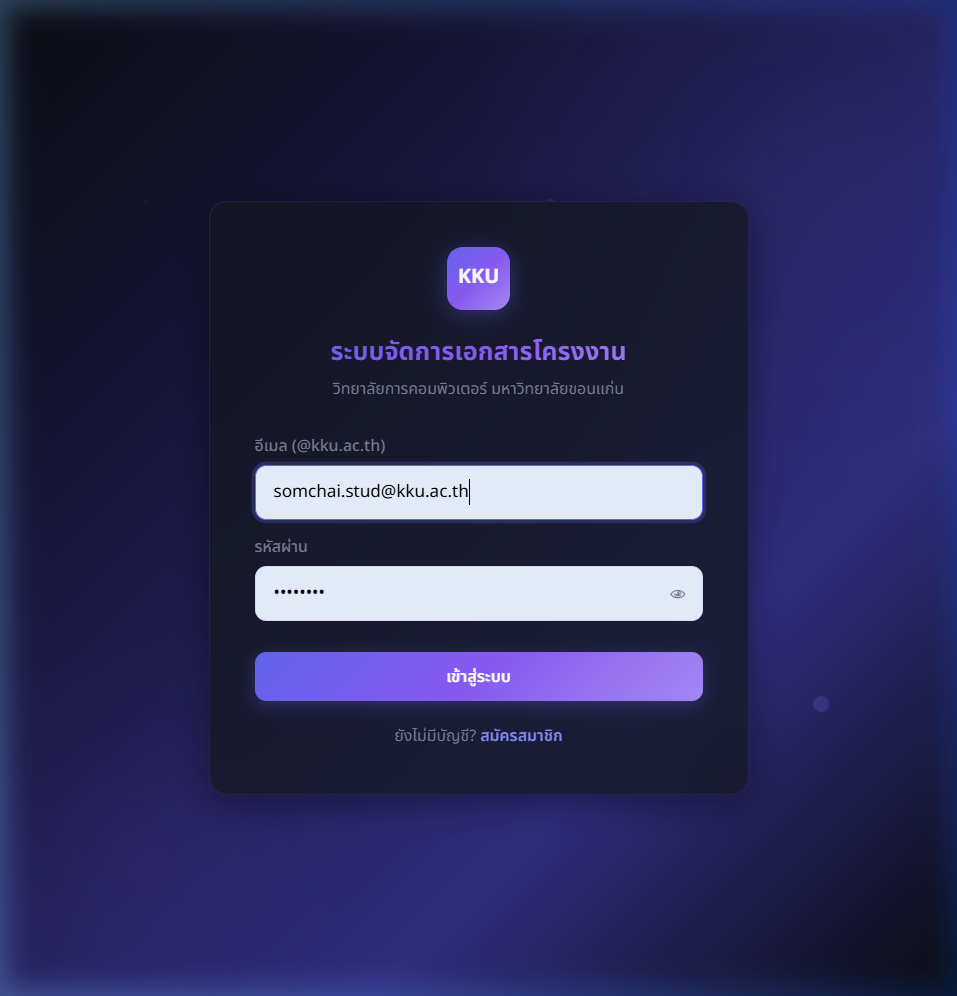
\includegraphics[width=0.8\textwidth]{images/ui-login.png}
\fbox{\parbox{0.75\textwidth}{\centering\vspace{4cm}\textit{แทรกภาพหน้าจอ Login ที่นี่}\\ใช้คำสั่ง \texttt{\textbackslash includegraphics}\vspace{4cm}}}
\caption{หน้าจอเข้าสู่ระบบ (Login)}
\label{fig:ui_login}
\end{figure}

หน้าจอหลัก (Dashboard) แสดงดังภาพที่ \ref{fig:ui_dashboard}

\begin{figure}[H]
\centering
% 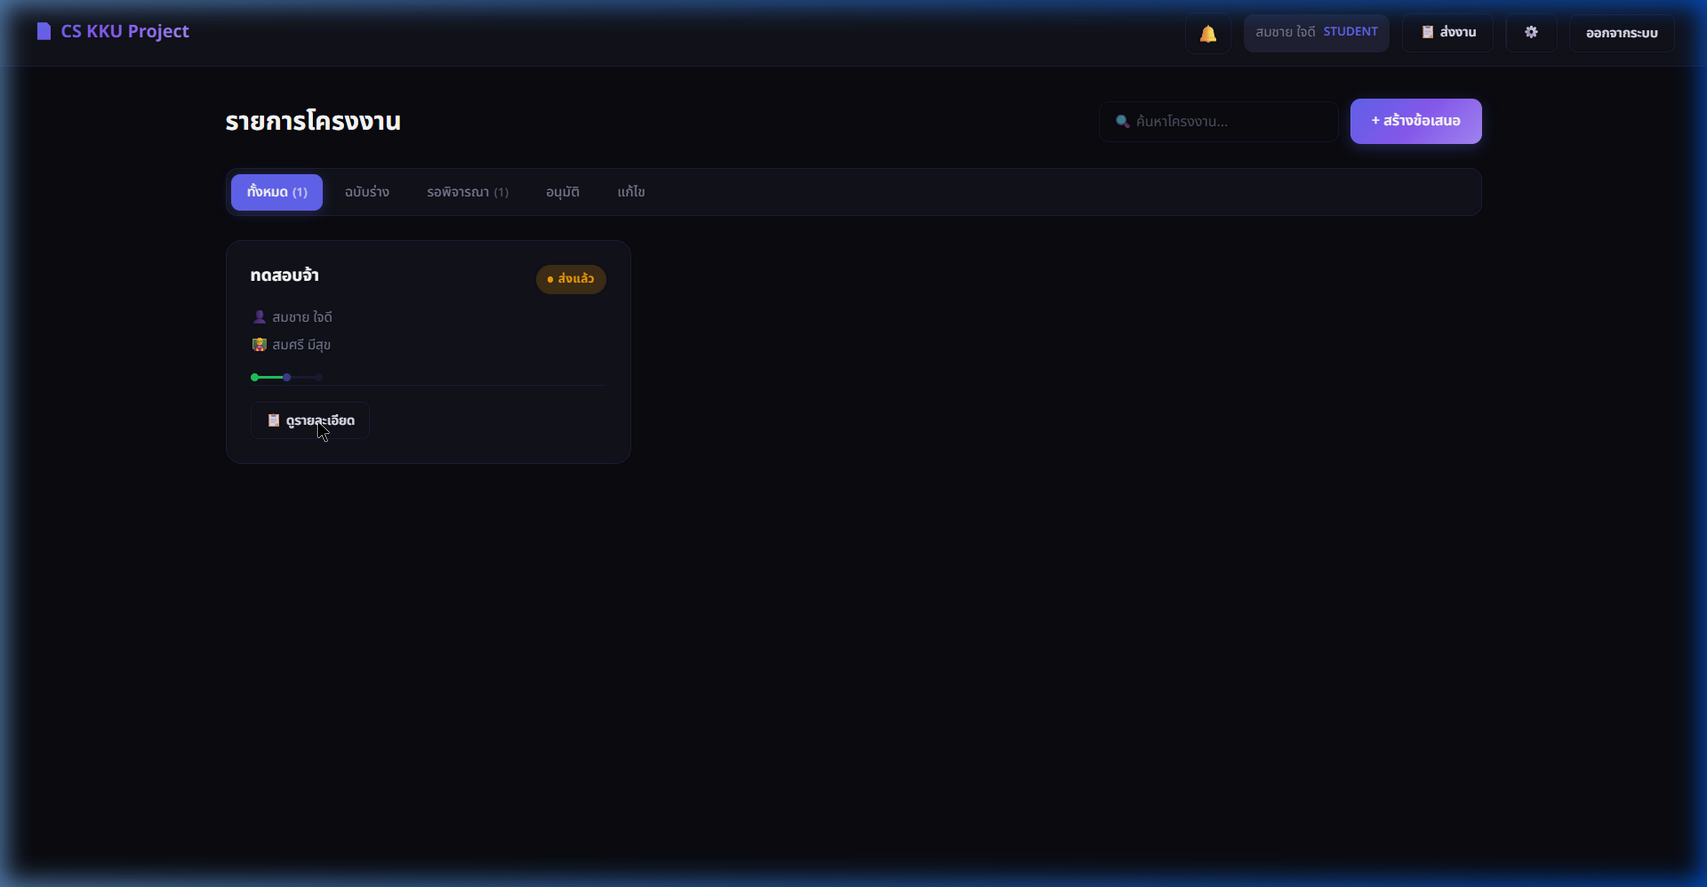
\includegraphics[width=0.8\textwidth]{images/ui-dashboard.png}
\fbox{\parbox{0.75\textwidth}{\centering\vspace{4cm}\textit{แทรกภาพหน้าจอหลักที่นี่}\vspace{4cm}}}
\caption{หน้าจอหลัก (Dashboard)}
\label{fig:ui_dashboard}
\end{figure}

\section*{คู่มือการใช้งาน}

อธิบายขั้นตอนการใช้งานระบบโดยสังเขป\ldots{}

% =============================
% ภาคผนวก ข
% =============================
\appendiceschapter{ความไวของพารามิเตอร์ Elo}

\section*{วิธีการ}

ค่า $K$ (ขนาดการปรับ) และ $h$ (ความได้เปรียบของเจ้าบ้าน) ของระบบ Elo ในหัวข้อการคำนวณคะแนน Elo ถูกเลือกบนข้อมูลที่อยู่ก่อนข้อมูลที่ใช้ฝึกและทดสอบแบบจำลองทั้งหมด ภาคผนวกนี้ทำการค้นหาซ้ำเพื่อให้ตรวจสอบได้ ดังนี้

\begin{enumerate}[label=\arabic*)]
    \item ใช้ผลการแข่งขันลีกของ 5 ลีกใหญ่จาก Football-Data.co.uk ฤดูกาล 2000--2001 ถึง 2014--2015 รวม 26,946 นัด โดยฤดูกาล 2000--2001 ถึง 2004--2005 ใช้เพียงอุ่นคะแนน Elo ให้เข้าที่
    \item คำนวณ Elo ใหม่สำหรับทุกคู่ $K \in \{5, 10, 15, 20, 25, 30\}$ และ $h \in \{0, 20, 40, 60, 80, 100\}$
    \item ทำนายผล H/D/A ด้วยแบบจำลองจำนวนประตู Poisson ที่ใช้ผลต่าง Elo เป็นตัวแปรเดียว แบบ Walk-forward บนฤดูกาล 2005--2006 ถึง 2014--2015 (18,260 นัด) โดยแต่ละฤดูกาลทำนายจากแบบจำลองที่ฝึกด้วยฤดูกาลก่อนหน้าเท่านั้น
\end{enumerate}

ผลสร้างซ้ำได้ด้วยคำสั่ง \texttt{uv run elo\_sensitivity}

\section*{ผลการทดสอบ}

\begin{table}[H]
\centering
\caption{Walk-forward Log Loss ฤดูกาล 2005--2006 ถึง 2014--2015 ตามค่า $K$ (แถว) และ $h$ (คอลัมน์) ตัวหนาคือค่าที่ใช้ในโครงงาน}
\label{tab:elo_sensitivity}
\begin{tabular}{|c|c|c|c|c|c|c|}
\hline
$K$ \textbackslash{} $h$ & 0 & 20 & 40 & 60 & 80 & 100 \\
\hline
5 & $0.9972$ & $0.9972$ & $0.9973$ & $0.9975$ & $0.9976$ & $0.9978$ \\
10 & $0.9942$ & $0.9942$ & $0.9943$ & $0.9943$ & $0.9944$ & $0.9945$ \\
15 & $0.9941$ & $0.9941$ & $\textbf{0.9941}$ & $0.9942$ & $0.9942$ & $0.9942$ \\
20 & $0.9950$ & $0.9950$ & $0.9950$ & $0.9950$ & $0.9950$ & $0.9949$ \\
25 & $0.9962$ & $0.9962$ & $0.9962$ & $0.9962$ & $0.9961$ & $0.9960$ \\
30 & $0.9976$ & $0.9976$ & $0.9976$ & $0.9975$ & $0.9975$ & $0.9973$ \\
\hline
\end{tabular}
\end{table}

ค่าที่ใช้ ($K = 15$, $h = 40$) ให้ Log Loss $0.9941$ เท่ากับค่าต่ำสุดของตาราง ค่า $h$ แทบไม่มีผล (ต่างกันไม่เกิน $0.0001$ ในแถว $K = 15$) เนื่องจากแบบจำลองจำนวนประตูเรียนรู้ความได้เปรียบของเจ้าบ้านจากค่าคงที่ของตัวเองอยู่แล้ว ส่วน $K$ ระหว่าง 10--20 ให้ผลต่างกันไม่เกิน $0.001$ และแย่ลงเมื่อ $K$ เล็กเกินไป (คะแนนปรับตัวช้า) หรือใหญ่เกินไป (คะแนนแกว่งตามผลนัดล่าสุด) การดึงคะแนนกลับสู่ค่าเฉลี่ยตอนต้นฤดูกาล (Season Regression) ร้อยละ 10, 20 และ 30 ให้ Log Loss $0.9944$, $0.9950$ และ $0.9958$ ตามลำดับ จึงไม่ได้ใช้

ผลนี้แสดงว่าข้อสรุปของโครงงานไม่ได้ขึ้นกับการเลือกค่าพารามิเตอร์ Elo ที่พอดีกับข้อมูล


% ==========================================
% ประวัติผู้เขียน
% ==========================================
\begin{biography}
% ประวัติผู้เขียน
% หมายเหตุ: ไม่เกิน 1 หน้ากระดาษ
%
% *** ลบข้อความตัวอย่างด้านล่าง แล้วเขียนประวัติของตนเอง ***

\section*{นักศึกษาคนที่ 1}

นาย/นางสาว\ldots{} เกิดเมื่อวันที่\ldots{} ที่\ldots{}
สำเร็จการศึกษาระดับมัธยมศึกษาตอนปลาย จากโรงเรียน\ldots{} เมื่อปีการศึกษา\ldots{}
ปัจจุบันกำลังศึกษาระดับปริญญาตรี หลักสูตรวิทยาศาสตรบัณฑิต
สาขาวิชาวิทยาการคอมพิวเตอร์ วิทยาลัยการคอมพิวเตอร์ มหาวิทยาลัยขอนแก่น

% ถ้ามีรางวัลหรือทุนการศึกษา:
% ได้รับ ... จาก ... เมื่อ พ.ศ. ...

% ถ้ามีประสบการณ์ทางวิชาการ:
% มีประสบการณ์ ...


% --- uncomment ด้านล่างนี้ ถ้ามีนักศึกษาคนที่ 2 ---
% \section*{นักศึกษาคนที่ 2}
%
% นาย/นางสาว\ldots{} เกิดเมื่อวันที่\ldots{} ที่\ldots{}
% สำเร็จการศึกษาระดับมัธยมศึกษาตอนปลาย จากโรงเรียน\ldots{} เมื่อปีการศึกษา\ldots{}
% ปัจจุบันกำลังศึกษาระดับปริญญาตรี หลักสูตรวิทยาศาสตรบัณฑิต
% สาขาวิชาวิทยาการคอมพิวเตอร์ วิทยาลัยการคอมพิวเตอร์ มหาวิทยาลัยขอนแก่น

\end{biography}

\end{document}